\subsection{Quadrant III. (Explicit Assurances, Informal Trust Treatment)}\label{sec:q3}
\subsubsection{Performance Prediction} \label{sec:performance_prediction}
    \citet{Zhang2014-he} are concerned with the performance of visual classification systems; particularly with the common occurrence of vision systems to fail `silently', that is with no warning. They suggest that the two possible solutions are to: 1) analyze the output of the vision system to assess its confidence, and 2) analyze the input itself in order to assess the classifier's confidence. They pursue the second, with the goal of minimizing failures as well as trying to verify the safety of a classifier. They argue that the second method is more desirable because it can be applied to any classifier. In essence they learn a model of the training error associated with different images and then use this to predict the error on test images. They demonstrate their methods on several different classification tasks and show that it predicts failure ``surprisingly reliably''. Although, they make an assumption that similar inputs (by some measure) will give similar outputs, which can be difficult to quantify in some domains.

    \citet{Gurau2016-hs} (following from ideas in \citet{Churchill2015-ei}) consider the task of predicting the performance of a robot's navigation when using cameras for localization. Their aim was to have the robot operate autonomously only when it was confident that it could do so, otherwise it would request human assistance. To achieve this they make use of GPS localized observations and `Experience Based Navigation' (EBN) to identify which past experience matches the current state of the robot. Using this approach they are able to reduce the number of mistakes that the robot makes when navigating in a real scenario. This approach seems to be fairly sound in their suggested application, and they claim that it is agnostic of classifier, which should be beneficial for use in other AIAs.

    \citet{Kaipa2015-hy} also consider the confidence of a visual classifier, but with the application being a robot that is picking an object out of a bin. To do this they utilize the `Iterative Closest Point' (ICP) method to match which points in a point cloud are likely associated with the object of interest in the bin. With that information the robot can then asses how confidently it can perform the task and if its confidence is below some threshold it will request assistance from a human. This method is quite similar to `Chi-square innovation hypothesis testing' used for adaptive Kalman filtering \cite{Bar-Shalom2001-tg}, and shares a key drawback, which is that it requires a precise model, and doesn't necessarily indicate \emph{why} the test is failing. Regardless, if applicable they are quite useful for verifying that the AIA is `OK'.

    \citet{Kuter2015-qh} recognize that plans produced by hierarchical tasking networks can be fragile, and suggest that the planner calculate its stability. In essence, how sensitive is the plan to uncertainties? They suggest `counter planning' and `plan repair' so that the autonomous system can identify likely contingencies that might interfere with an existing plan and then adapt the plan to account for those contingencies. If the system \emph{is} able to adapt to contingencies then it will have a higher `self-confidence'. This allows humans to be able to understand the system better, and trust it more appropriately.

    \citet{Hutchins2015-if} consider the fact that autonomous systems have components, and that those components have `competency boundaries'. Which refers to the fact that different sensors, planners, and actuators have different capabilities in different conditions. For example a GPS has high competency in an open-air situation, but very low competency inside of a tunnel or building. They suggest that these competency boundaries be quantified, and then displayed to a user, so the user better understands the system's capabilities and can trust it more. The main limitation here is that they propose an expert-based Likert scale for quantifying competency boundaries, which, which  lacks formal foundations, and extensions to other domains. Both this work and that of \citeauthor{Kuter2015-qh} are related to the work of \citeauthor{Aitken2016-fb}, but the later two do not explicitly relate their approaches to trust and TRBs. Although, \citeauthor{Hutchins2015-if} is the only paper of the three to consider the exact method by which the assurance should be communicated.

\subsubsection{Interpretable Models} \label{sec:model_interp}
    A well-known concept in machine learning and pattern recognition is the trade-off between accuracy and interpretability. \citet{Van_Belle2012-dt} examine this issue in the context of making clinical decision support systems for use in the medical field. To this end they propose an `interval coded scoring' system that imposes a constraint such that each variable has a constant effect on the estimated decision-making risk (e.g. the Bayes' risk for classification).  They demonstrate the method on two datasets, and show that their method can be visualized using scoring tables and color bars. They point out that their method needs to be extended in order to detect interaction effects automatically, and to handle multi-class decision support systems. One reason why this approach is important is because probabilities are notoriously difficult for humans to interpret, and thus the reason to manipulate the output in order to accommodate those who interact with the system.

    Along these lines,  \citet{Ruping2006-xj} specifically asks how classification results can be made more interpretable to those who design and use classifiers. He reviews several possible methods, and states that ratings by experts is perhaps the most accurate way, although it is at the same time subjective. To address the accuracy-interpretability trade-off he investigates the use of a simpler global model, and a more complex local model (\citet{Otte2013-oo} and \citet{Ribeiro2016-uc} implement similar ideas as well). Figure \ref{fig:ruping} illustrates this idea on a simple example, the left (global) model can be used as a large scale interpretable model, while the more complex local model can be used as necessary when more precise understanding is required. This allows simple interpretation of global properties, but more complex local models to maintain accuracy. While his focus was on classification, the methods could also be useful in regression as well. He spends time investigating how the global and local models should be learned in a principled way, and demonstrates this approach on several black-box and white-box classifiers. 

    \begin{figure}[htbp]
    \centering
    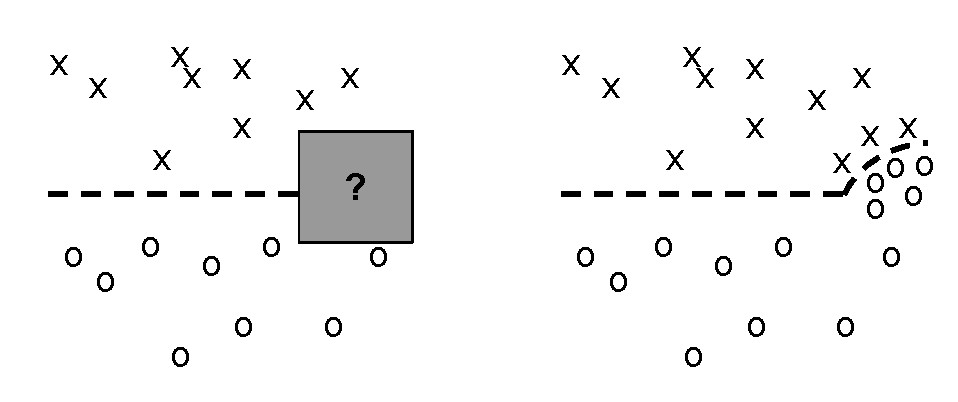
\includegraphics[width=0.8\textwidth]{Figures/global_local}
    \caption{Example of simple global model on the left, and on the right a more complex local model that can be used for interpretability when more detail is necessary.}
    \label{fig:ruping}
    \end{figure}

    Later, \citet{Van_Belle2013-ph} address the challenge that some of the highest performing ML models are too complicated to be interpreted. They investigate different `interpretable' and visualization methods in order to understand what opportunities they find. They suggest that there are three methods that help ascertain the level of interpretability and potential utility of models: 1) Map to domain knowledge, 2) Ensure safe operation across the full operational range of model inputs, and 3) Accurately model non-linear effects (compare to categories proposed by \citet{Lipton2016-ug}). They analyze some of the existing methods (nomograms, rule induction, graphical models, data visualization) and point out their weaknesses. They finish by pointing to more recent research in sparse and interpretable models, and suggest that it is a promising line of research. In summary, they discuss that each `interpretable' method has its benefits and weaknesses and there is no method that clearly out-performs any other.

    Similarly, \citet{Caruana2015-za} are interested in predicting the probability that a patient will be re-admitted to the hospital within thirty days. They also mention the trade-off between accuracy and interpretability, and propose a generalized additive model with pairwise interactions ($GA^2M$) model. A generalized additive model (GAM) is generally thought of as interpretable as the effects of individual variables can easily be quantified; however GAMs suffer from low accuracy. In a comparison with other methods, they show that adding pairwise interactions allows the $GA^2M$ model to be as accurate as the current less interpretable methods, while still maintaining reasonable interpretability.

    In a similar vein, \citet{Choi2016-by} modify a recursive attention neural network to remove recurrence on the hidden state vector, and instead add recurrence on the doctor visits and diagnoses. In this way the model is able to predict possible diagnoses in time, and a visualization can be that that indicates the critical visits and diagnoses that lead to that prediction. These methods are promising because it restructures an advanced learning model in a way that useful information can be extracted. This method seems very promising, however, their architecture is dependent on problems with similar properties, meaning that their approach would need to be re-implemented by an expert to be used in another situation.

    \citet{Abdollahi2016-vn} construct a conditional restricted Boltzmann machine (RBM) in order to create a collaborative filtering algorithm, that can suggest `explainable' items, while maintaining accuracy. The challenge is that the RBMs are very accurate collaborative filtering algorithms, but difficult to understand. They make a more explainable version by adding an additional `explainability layer' which indicates the explainability of an item to a certain user. This method shows how adding an additional element in a model can help add explainability, and this seems to be somewhat of a theme in this section.

    \citet{Ridgeway1998-lv} recognize that boosting methods, or classifiers with voting methods, are very accurate but not interpretable. They propose boosting by `weight of evidence' (WoE), where WoE refers to having a weight that indicates whether the observation is positively or negatively correlated to the class. Each weight can then be used to gain some understanding about how the observation affects the classification. They demonstrate its utility using multiple experiments that it has performance on par with AdaBoost, and with a Naive Bayes classifier.  Again, their approach gets at the ability of adding in interpretability components into a model can yield a more interpretable model, while losing very little accuracy.

    \citet{Huysmans2011-th} investigate decision trees, decision tables, propositional if-then rules, and oblique rule sets in order to understand which is the most interpretable and perform an experiment to identify which method works most effectively. The experiment involved interpreting a model and answering questions about what the correct classification would be. They made several interesting observations. First, they confirmed that a model with larger representation leads to lower answer accuracy responses. They found that overall decision trees and decision tables were the most interpretable, but that different tasks made the tree or table more desirable (the layout of the data in a table can be superior for certain `look-up' tasks). 

    One drawback with decision trees is that the rules can get very complicated in a large tree. \citet{Park2016-ld} investigate how to make rules in decision trees more `intuitive'. They propose a method that learns chains of decisions that together increase the ratio of positive class. They present a method that is called $\alpha$-Carving decision Chain (ACDC), and say that it is a greedy alternative to a general framework known as RuleLists (\citet{Wang2015-ww}). Similarly, \citet{Jovanovic2016-gw} use `Tree-Lasso' logistic regression with domain knowledge. Specifically they use medical diagnostic codes to group similar conditions and then use `Tree-Lasso' regression that uses that information to make a more sparse model. \citet{Zycinski2012-jj} also use domain knowledge to structure the data matrix before feature selection and classification. While the work of \citeauthor{Huysmans2011-th} gives some indication about how to choose classifiers for interpretability, \citeauthor{Park2016-ld} points out that to gain \emph{real} interpretability in complex tasks expert knowledge is still needed to make sense of complicated features.

    \citet{Faghmous2014-og} argue that `theory guided data science' is necessary in science applications; for instance, when studying environmental effects, black-box models are of little use. Instead, in order to gain insight they need a theoretical framework, to help highlight causation. Similarly, \citet{Morrison2016-fz} address the situation where an analytical model is available but imperfect. They use a chemical kinetics application where the theoretical reaction equations are well known, and then add a `stochastic operator' over the top of the known model to account for uncertainties. One drawback for these methods is that they require a lot of domain knowledge. However, in the areas of science and engineering where physical models are well understood this type of approach could be useful to indicate the performance of the system with regards to the theoretical model.

\subsubsection{Visualization and Dimensionality Reduction} \label{sec:viz_dr}
    Intuitively, it might make sense to simply show users the inputs, raw data, and/or intermediate processing steps that led to a particular AIA behavior. In many real applications, however, there are too many individual variables for a human to attend to. In such situations, dimensionality reduction (DR) and visualization are tools that can be used to help make a model or data easier to understand. \citet{Venna2007-yj} discusses dimensionality reduction as a tool for data visualization for ML, and reviews many linear and non-linear projection methods. \citet{Vellido2012-nm} also discusses the importance of DR for making ML models interpretable.

    In an interesting application to time series data, \citet{Kadous1999-rx} asks how comprehensible descriptions of multivariate time series can be learned, with the end goal of interpreting Australian sign language. He focuses on reducing the feature space fed into a learning algorithm (i.e. the data was gathered using an instrumented glove), and does so using `parameterized event primitives' (PEPs), which are commonly occurring events or patterns that are expected to occur. He shows that his method reduced test error while also having more comprehensible features. It seems likely that parameterized primitives might be automatically learned. While an interesting application, this would require expert knowledge to extend to other domains. Although it does seem likely that PEPs could be automatically identified in some way.

\subsubsection{Explanation} \label{sec:explanation}
    In the context of POMDP planning, \citet{Lomas2012-ie} recognize that in order for humans to appropriately trust robots they must be able to predict their behavior, and the robot must be able to communicate in order for that to happen. To this end they present the Explaining Robot Actions (ERA) system that interfaces with a model that represents semantic and physically based information, along with other factors. In essence the ERA is a translator between the planner/model and the human. This approach depends on a layered world model that includes semantic information as well as the physical model, but is promising in the respect that the ERA is a separate system that queries the robot. 

    With regards to expert systems \citet{Swartout1983-ko} examines explanation methods. He noted that ``trust in a system is developed not only by the quality of its results, but also by clear description of how they were derived''. Often the data (or knowledge) used to train an expert system is not kept in the system for later use. He proposed a method called `XPLAIN' that not only describes \emph{what} it did, but \emph{why} it did it. It does this by using description facts of the domain and prescriptive principles simultaneously; in essence it learns how to make decisions and how to explain them at the same time. This approach is meant for a  structured problem defined by a domain model and the domain principles, in situations where problems are based mostly in data, this approach would not be applicable.

    \citet{Rouse1986-dz} asked how computer-based decision support systems should be designed in order to help humans cope with their complexity. He suggests that methods need to be designed so as to provide different kinds of information which include: patterns vs. elements, and current vs. projected outcomes or states. This work is important in pointing out that assurances also depend on what the role of the human is and what information they need.

    This was also investigated to some extent by \citet{Wallace2001-fm} in their work concerning explaining outcomes of constraint solvers. They discuss how to distinguish between `good' and `bad' explanations, or those explanations that facilitate or detract from the user's ability to understand how the explanation actually applies to the solution being explained. They critically ask the question of how explanations should be presented to users (something that \citet{Kuhn1997-qc} explores more formally with regard to framing of uncertain information in decision making). An important consideration is that constraint solvers don't take uncertainty into account, but instead are deterministic. This is not the case in many of the more adaptable and capable AIAs.

    \citet{Lacave2002-cu} revisit some of these ideas from the perspective of explaining Bayesian networks. They are concerned with \emph{how} and \emph{why} a system reaches a conclusion. They present three properties of explanation: 1) content (what to explain), 2) communication (how to explain), and 3) adaptation (how to adapt based on who the user is). It is not possible to cover all of the ideas that they present in their paper, but they are key to the idea of designing assurances. Some key points are that they highlight the differences between explaining evidence, the model, or the reasoning. These are three key considerations in making assurances. They also discuss whether an explanation is meant to be a description or for comprehension, as well as whether explanations need to be on a macro or micro scale (as mentioned by \citeauthor{Ruping2006-xj}). They also consider whether explanations should occur by two-way interaction between system and user, by natural language interaction, or by probabilities. Finally, when considering adaptation, they hit on another key point of assurances, which is that in general application not all users will require (or desire) the same kinds of assurances. This paper points out many challenges and considerations in designing assurances, and illustrates that, as with the `No free lunch' theorem, there is no single `best' assurance that will address every possible situation.


\subsubsection{Model Checking} \label{sec:model_checking}
    While assurances behind reasoning processes can be useful in many situations, they are not trustworthy in and of themselves if the models or assumptions they are based on are flawed to begin with. Thus, there is also great interest in providing assurances that the models and assumptions underlying said AIA reasoning processes are, in fact, sound. \citet{Laskey1991-mf} -- with the intention of helping users of `probability based decision aids' by communicating the validity of the model -- notes that it is infeasible to perform a decision theoretic calculation to decide if revision of the model is necessary. She then presents a class of theoretically justified model revision indicators which are based on the idea of constructing a computationally simple alternate model and then to initiate model revision if the likelihood ratio of alternate model becomes too large. 

    \citet{Zagorecki2015-qy}, discusses the `surprise index' introduced by \citet{Habbema1976-xd}, which is the likelihood of a certain measurement given a specific model, which applies nicely to Bayes-nets that have probabilistic descriptions. The major flaw of the surprise index is that it is computationally infeasible due to the possibility (likelihood) of being a non-analytic distribution. \citeauthor{Zagorecki2015-qy} suggest an approximation by using the log-normal distribution to approximate the distribution of values in the joint probability distribution. Another challenge is knowing what a `good' value for the surprise index is since knowing the maximum likelihood of a non-analytic distribution is not an easy problem.

    \citet{Ghosh2016-dl} present a method, in the framework of a practical self-driving car problem, called Trusted Machine Learning (TML). The main approach of TML is to make ML models fit constraints (be trustable). To do this they utilize tools from formal methods to provide theoretical proof of the functionality of the system. They present `model repair' and `data repair' that they can utilize when the current model doesn't match the data, at which point the model and data can be repaired and control can be replanned in order to conform with the formal method specifications. One challenge that presents itself is how to identify the `trustable' constraints, this returns a lot of responsibility to the designer to foresee all possible failures, which is a strong assumption.

\subsubsection{Human-Involved Learning} \label{sec:human_involved}
    Another possible way to make system assure a human user is to use the human in the learning process. \citet{Freitas2006-qo} addressed this point with regards to discovering `interesting' knowledge from data, by comparing two main approaches. Given such large datasets, human users require assistance from complex systems in order to find patterns and other `interesting' insights. He mentions `user-driven' methods that involve a user pointing out `interesting' templates, or in another method general impressions in the form of IF-THEN rules. He compares these methods to other `data-driven' methods that have been used, and cites other research that suggests that data-driven approaches are not very effective in practice. This is a cautionary tale that many times engineering methods to assist humans are not as effective as we would like to believe. Although, the `user-driven' approach may not fair any better when compared over many users, as each user will likely have different preferences. \citet{Chang2017-kl} also consider a similar, scaled up, `user-driven' approach called `Revolt' that crowd-sources the labeling of images. It is able to attain high accuracy labeling, while also exploring new or ambiguous classes that can be ignored with traditional approaches.

\subsubsection{Explicit Assurances via Formal Methods} \label{sec:VV}
    Validation and Verification (V\&V) typically refers to using formal methods to guarantee the performance of a system within in some set of specifications. Not all practitioners are aware that V\&V provides ways to assure users; arguably some have this idea in their mind, but only a few V\&V researchers consider how to communicate the results of analysis via formal methods to users. A prime example is given by \citet{Raman2013-mz}, who developed a way by which a user can provide natural language specifications to a robot and a `correct-by-construction' controller will be built if the specification is valid. Otherwise, the robot will provide an explanation about which specification(s) cause failure. They study this with the goal of implementing the system on a robot assistant in a hospital. Their method involves parsing natural language input (such as: ``Go to the kitchen''), and converting that to linear temporal logic (LTL) that represents a task specification. This is then used to construct a controller if possible, otherwise the `unrealizable' specifications need to be communicated back to the user. This approach is promising in that it presents a way to communicate that a specification cannot be met, although it does not formally account for effects on user trust or TRBs in formulating explanations. The expression of assurances is also asymmetrically limited to cases where the robot cannot meet the specifications. 

\subsubsection{Summary}
    Many of the approaches above focus on informing the user how the model/logic works; there is also some focus on predicting future performance. Some AIAs do not have the capability to implement these approaches. Or, the type of approach -- such as informing the user how a deep neural network works -- simply does not have a satisfactory answer to date. As another example, methods for quantifying the amount of uncertainty in a planner have not been developed for all planning algorithms. Likewise, there may not be satisfactory ways of visualizing certain data. %%In short, there is much work still to be done in order to design assurances for different AIA capabilities.

    The approach of using a more simplistic global model paired with more accurate local model is fairly prominent (\cite{Ruping2006-xj,Ribeiro2016-uc,Otte2013-oo}). This idea is similar to how human experts explain approaches to non-experts; as a non-expert desires to know more about a specific concept of a complex idea, more detailed explanation can be provided. This is promising because it is also extensible to different types of users. In particular \cite{Ribeiro2016-uc} is designed to work with any classifier, and \cite{Zhang2014-he} has the same goal as well. Of course the trade-off of accuracy for flexibility will always exist between more general approaches and specialized approaches.

    The underlying hypothesis here is that many of the methods should affect the user's perception of the `competency', and `predictability' of the AIA, or the `situational normality' of the task being performed. However, none of this has been tested by experimentation that gathers self-reported changes in trust. Similarly, there has been no formalization of how the effects of assurances on TRBs might be quantified in different applications. In essence this work is only addressing at a small subset of important considerations for designing assurances, or the subset that includes the methods by which to calculate the assurance. The experimental testing of the effects of the proposed assurances on both self-reported trust, and TRBs remains open. Indeed, the research in this section is mainly focused on what AIA engineers and designers \emph{think} needs to be explained, or what assurance they \emph{think} users should have. These ideas definitely have merit, but need to be tested to identify if they are effective, to what extent they are effective, and whether there is a more effective, or more efficient way to achieve similar results.
